\documentclass[10.7pt]{article} % 11pt article, want AMS fonts.

\usepackage{amsmath,amsfonts,amssymb}
\usepackage{latexsym}
\usepackage{hyperref}
\usepackage{graphicx}
\graphicspath{ {./images/} }
\usepackage{setspace}
\usepackage{blindtext}
\usepackage[a4paper, total={6in, 8in}]{geometry}
\usepackage[demo]{graphicx}
\usepackage{subfig}
\usepackage{indentfirst}
\usepackage{changepage}
\usepackage{booktabs}
\usepackage{array}
\usepackage{mathtools}
\usepackage[hang,flushmargin]{footmisc} 
\date{}

\textheight=8in					% Body height (incl. footnotes)
\skip\footins=1ex				% Space above first footnote.

% \singlespacing
% \onehalfspacing
\spacing{1.2} %to change spacing if necessary 

\begin{document}

\title{How Much Is A Best Picture Oscar Worth?}
\author{Aryan Arora, Isabella Cha, Kevin Phung}
\maketitle

\section{Introduction}
The Academy of Motion Picture Arts and Sciences granted the first Oscars in 1929, creating what is today the oldest, most visible, and most prestigious award in the film industry (Levy 2001). The Academy Awards, now officially the Oscars, has changed little since 1929 - the nominees and winners are still decided by the members of the Academy, the nominees are revealed a month or two before the awards ceremony, and the winners are announced at the ceremony.

The existing literature suggests that movies are “experience goods” defined as “products which consumers choose, buy and use solely to experience and enjoy” (Sawhney and Eliashberg 1996). The intangible and experiential nature of movie consumption makes it difficult to judge movie quality before it is actually viewed; as such, consumers may seek other signals prior to the consumption experience (Bristor 1990; Harrison-Walker 2001; Y. Liu 2006). The Oscars, arguably the most important award in the movie industry, is thought to be an important signal in shaping consumer perceptions (Ginsburgh 2003). The movies that receive this honor go down in history as films of quality and prestige. As noted by Levy (2001), “No other award so well combines critical and popular judgment”. Through the Oscars, the Academy functions as peers, critics, and tastemakers — thus, the question of how much an Oscar is worth is a pertinent one. 

In this paper, we are particularly concerned with the ‘Best Picture’ award, the highest honor of the ceremony. We define “worth” as commercial success, as measured by box office revenues. We will use econometric tools to measure whether winning a Best Picture Oscar increases consumers’ demand for a movie by significantly increasing weekly box office revenues. Our results show that Best Picture nominations boost movies’ revenues, whereas the effect of a win is not significant.  



\section{Theoretical Framework}
A movie’s box office revenue is directly related to the number of consumers purchasing tickets to view the movie. Economic theory suggests that the number of tickets sold is a function of consumer demand for seeing a given movie. Factors affecting consumer’s demand are likely to include the number of theaters, theater run, budget, genre, rating, whether the movie features a “star,” and if the film released around a holiday. 

\subsection{Determinants of Movie Demand} 
\setlength\parindent{0pt}

\begin{adjustwidth}{1cm}{}

\textbf{Number of theaters} \newline
More theaters implies that consumers have easier access to see a given movie; if a moviegoer is deciding between different movies, all else equal, then they are more likely to see the one screening closest to them. Additionally, some consumers may not decide what to watch until entering the theater. Then, all else equal, the likelihood of watching a movie increases as the movie is shown in more theaters. \\


\textbf{Budget}\newline
A larger budget might improve movie quality through better camera equipment, higher quality editing, and better sound. In addition, a larger budget allows for more spending on advertising and promotion which might also increase demand. Previous studies suggest that large budget films generate more revenue (Deuchert et. al 2005), though there is no consensus on the elasticity between movie expenditures and revenue.  
\\

\textbf{Genre}\newline
 Film genres appeal differently to different moviegoers. For example, animated and family films are the most popular genre for children accompanied by parents, action/adventure films appeal to younger audiences, and dramas are more popular among older audiences (Redondd and Holbrook 2010). A movie’s strongest competition comes from other movies that are most alike in genre (Elberse 2005; Y. Liu 2006). From this, we postulate that movies in the same genre category may be substitutes; all else equal. Then more substitutes decrease demand for a particular film. 
 \\

\textbf{MPAA Rating}\newline
The MPAA rating of movies may attract or repel certain audiences. G and PG rated movies may be more appealing to families, whereas R-rated movies may appeal to more mature audiences. However, the effect of MPAA ratings may be ambiguous: for instance, the presence of obscene language, explicit sex, and/or violence was reported as the second most important factor in avoiding R-rated movies (Moon et al. 2010). On the other hand, some studies suggest sexual content is intrinsically profitable precisely \textit{because} of its controversial nature (Pennington 2007). \\

\textbf{Holiday}\newline
Whether or not a movie was released around a holiday may be a determinant of movie demand. The number of moviegoers varies dramatically throughout the year according to Einav (2007), who observes a “seasonal pattern” of movie sales, with the biggest hits in the beginning of the Christmas holiday season. However, it is also plausible that consumers may prefer to stay at home with family rather than go to movie theaters on Christmas. \\

\textbf{Star Power}\newline
Star power is considered to be one of the key drivers of motion picture success, albeit with some controversy. As Bill Mechanic, former chairman of Twentieth Century Fox put it, “a guy stranded on an island without Tom Hanks is not a movie… there's no way to replace that kind of star power.”  Elberse (2007) finds that on the basis of a multiple regression model, star power has no significant box office sales. On the other hand, Prag and Casavant (1994) found that star power and winning an Academy Award are “unambiguous positive factors in a movie’s financial success.” 
\end{adjustwidth}


\setlength{\parindent}{20pt}

\section{Data}
\subsection{Data Collection} 
Our dataset includes all Oscar-Best picture nominated movies that were released in the US after January 1, 2000, and which had an official domestic (US) running time that did not exceed December 31, 2019. In order to isolate the effect of the Oscar event, we excluded films that were not nominated. We also decided to exclude movies running from 2020 and beyond due to the COVID-19 pandemic and the shutdown of theaters. We then collected data for our dependent variable and possible explanatory variables as outlined in our theoretical framework. 

Weekly box office returns, release dates, and budget information are taken from boxofficemojo.com. To check whether awards influence success, we look at weekly revenue (as opposed to gross revenues) accounts for the income generated after the Oscars announcement, in order to be able to determine whether it is the Oscar announcement that triggered the additional income. It is also important to note that the industry operates on a weekly schedule --— much of the competition is over the weekend audience. Consequently, release dates are tabulated at the weekly level. 

Nominations, wins, details on genre, movie content ratings were taken from Internet Movie Database (IMDb). Additionally, data for movie budgets was scraped from The-Numbers (https://www.the-numbers.com/). Star power was constructed from Forbes' list of 100 Highest paid Actors and Actresses for each respective year. 

As final step, we merged and cleaned our datasets from various website using automated Python scripts. Our final dataset includes 125 movies and weekly revenue data for each movie. In total, we have 2999 observations. 

\setlength{\parindent}{20pt}

\section{Data}
\subsection{Data Collection} 
Our dataset includes all Oscar-Best picture nomianted movies that were released in the US after January 1, 2000, and which official domestic (US) running time did not exceed December 31, 2019. In order to isolate the effect of the Oscar event, we exclude films that were not nominated. We also decided to exclude movies running from 2020 and beyond due to the COVID-19 pandemic and the shutdown of theaters. We then collected data for our dependent variable and possible explanatory variables as outlined in our theoretical framework. 

Weekly box office returns, and release dates are taken from boxofficemojo.com. To check whether awards influence success, we look at weekly revenue (as opposed to gross revenues) to account for the income generated \textit{after} the Oscars announcement, in order to be able to determine whether it is the Oscar announcement that actually triggered the additional income. It is also important to note that the industry operates on a weekly schedule --— much of the competition is over the weekend audience. Consequently, release dates are tabulated at the weekly level. Budget data was taken from the-numbers.com. 
As the budget data we obtained was inflation adjusted, we also adjust our weekly box office revenues for inflation, by deflating the data by the Consumer Price Index (CPI) of 2000 as our base year. 

Nominations, wins, details on genre, movie content ratings were taken from Internet Movie Database (IMDb). Additionally, data for movie budgets was scraped from The-Numbers (https://ww w.the-numbers.com/). Star power was constructed from Forbes, List of 100 Highest paid Actors and Actresses for each respective year. 

As final step, we merged and cleaned our datasets from various website using automated Python scripts. Our final dataset includes 125 movies and weekly revenue data for each movie. In total, we have 2999 observations. 

\subsection{Description of Variables}

%Dep var %
\begin{table}[h]
\caption{Dependent Variable}
\label{tab:my-table}
\resizebox{\textwidth}{!}{%
\begin{tabular}{|l|l|}
\hline
\textbf{Variable Name} &
  \textbf{Description} \\ \hline
\textit{WeeklyEarnings} &
  \begin{tabular}[c]{@{}l@{}}Revenues from US ticket sales, measured in USD and adjusted for inflation. \\ Does not include DVD rentals, streaming purchases, or additional releases of the film.\end{tabular} \\ \hline
\end{tabular}%
}

\end{table}

% EXP VARS
\begin{table}[h]
\caption{Possible Explanatory Variables}
\label{tab:my-table}
\resizebox{\textwidth}{!}{%
\begin{tabular}{|l|l|}
\hline
\textbf{Variable Name}    & \textbf{Description}                                                   \\ \hline
\textit{CumulativeWeeks} & \begin{tabular}[c]{@{}l@{}}
Number of weeks after release, starting from 1. \\ Relevant because 
 ``novelty effect" may wear off over time. \end{tabular}              \\ \hline
\textit{GrossRevenueTilNom} & 
\begin{tabular}[c]{@{}l@{}}
Gross revenues up till the point of nomination.\\Tabulated at the weekly level.         \end{tabular}\\ \hline

\textit{WeeklyRank}      &
\begin{tabular}[c]{@{}l@{}} Rank of the movie (in terms of revenue) relative to other movies\\ showing in the same week across the US \end{tabular}   \\ \hline

\textit{NumTheaters\footnotemark}         & Number of cinemas showing the movie. Only includes US theaters.   \\ \hline

\textit{Budget}           & Movie production budget, measured in USD and adjusted for inflation.                     \\ \hline

\textit{MPAARating} (3 groupings) & \begin{tabular}[c]{@{}l@{}}(1) PG\\ (2) PG-13\\ (3) R\end{tabular}     \\ \hline

\textit{Genre\footnotemark} (5 groupings) &
  \begin{tabular}[c]{@{}l@{}}(1) Action, Adventure, Fantasy, Sci-Fi (AAFS); \\ (2) Drama,Comedy,Romance (DCR); \\ (3) Crime, Mystery, Horror, Thriller (CMHT); \\ (4) Biography, Sport, History, War (BSHW); \\ (5) Animation, musical, family (AMF); \\ Each genre grouping is a binary dummy variable indicating if \\the movie is classified as part of the grouping.
   
                       \\ \hline
  \end{tabular} \\ \hline
  
\textit{Holiday\footnotemark}  & 
   A binary variable to indicate if a movie is released in the holiday season. \\ \hline
\textit{StarPower\footnotemark}  &
  A binary variable to indicate if the movie has star power. \\ \hline
\textit{Nomination} & A binary variable if a movie was nominated for the Best Picture Oscar. \\ \hline
\textit{Win}        & A binary variable if a movie won the Best Picture Oscar.               \\ \hline
\end{tabular}%
}
\end{table}

\footnotetext[1]{In the correlation matrix, we refer to the num of theaters variable as 'Num\_T', everywhere else it is refered to as 'NumTheaters'}
\footnotetext[2]{In order to account for the dummy variable trap, we removed one category (Western) that was deemed multicollinear.}
\footnotetext[3]{Constructed variable. "Holiday season" is defined as the last 6 weeks of the calendar year.}
\footnotetext[4]{Constructed variable. A movie is classified as having star power if at least one of its main cast members appears in the \textit{Forbes List of 100 Top-paid Actors and Actresses} in their respective year of release. This classification is in similar fashion with previous studies done on star power \\(Liu Y. 2006; Liu, A. et. al 2014)}








\newpage
\subsection{Exploratory Data Analysis}

Prior to drawing up our model, we created a heat-map of a correlation matrix in an attempt to detect high levels of correlation between our explanatory variables. We found that most regressors did not have significant levels of correlation. We discuss a few important cases of correlation later in the paper.

\begin{center}
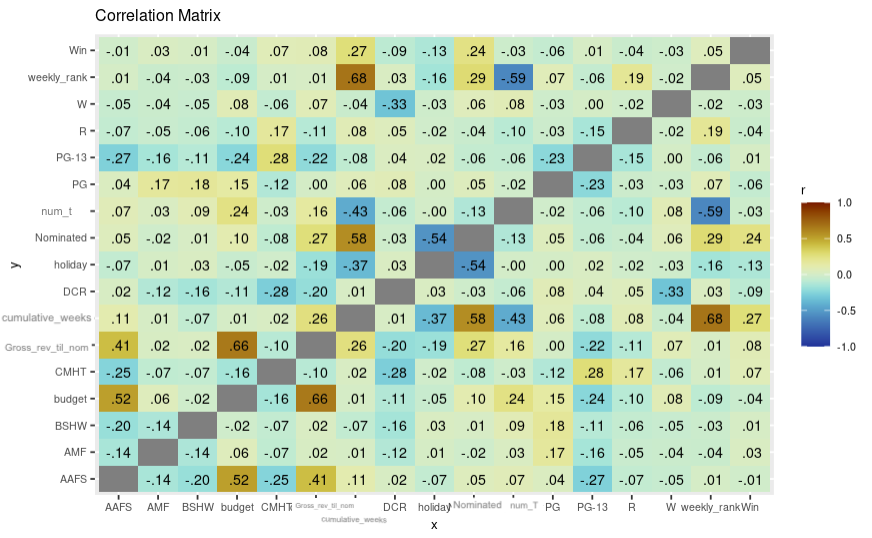
\includegraphics[scale=0.85]{version2/heatmap_fixed_labels.png}

\section{Model Specification}  
\end{center}

Given our economic theory for the variables we considered, we began by creating a model with all of our variables. We then ran F and T tests on the variables for which we did not have a strong enough economic theory and thus wanted to examine. We first ran an F test on both Genre and Ratings, for each of the sub-categories. This approach is a product of two considerations. The first is the risk of the omitted variable bias, the second is a comparatively larger risk of underfitting as compared to overfitting. Given the size of our dataset (roughly 3000 datapoints) we saw a much larger risk of underfitting and biasing our estimated (as shown by the ommited variable bias) as compared to overfitting. Thus we tried to include as many theoretically sensible variables as we could think of. We also included cumulative gross earnings and cumulative number of weeks variables because, working off our time series data, weekly revenues go down as films are out for longer periods of time (and receive more gross revenue). We ran tests on those we did not have substantial economic theory, or had controversial theoretical backing  (namely ratings, genre, star power, and an interaction between win and Gross Revenues till Nomination).

Our F test on Genre produced a statistically significant result at a 5\% significance level, with a p-value of 0.0009393. This meant that the restriction (removing the genre dummy variables) significantly worsened the goodness of fit. Hence, we kept all the genre dummy variables. 

Our F test on Rating did not produce a statistically significant result at a 5\% significance level (p value = 0.09054). This meant that the restriction (removing the rating dummy variables) did not significantly worsen the goodness of fit. Therefore, we decided to remove the rating dummy variables. 

Furthermore, the T test on the star power explanatory variable did not provide a statistically significant result at a 1\% level of significance. Given the opposing theoretical viewpoints on star power as a predictor of film earnings, we held a high threshold to include it in the model (hence 1\%), and thus we decided to omit the variable. We also removed the interaction between cumulative gross earnings and and win for similar reasons (p value = 0.88290).

Additionally, we then conducted tests for linearity and found non-linearity. We also ran a Ramsey Reset Test for a quadratic model. Our Reset statistic (RESET = 62.419, df1 = 12, df2 = 2972) provided evidence against the linear model, but we were inconclusive on the structure of the correct model. We attempted to resolve the non-linearity and incorrect model specification by logging the dependent variable: weekly earnings and budget and Gross Earnings till Nomination. Our residuals vs fitted values plots improved significantly and this provided the following Histogram and QQ plot of residuals: 

\begin{figure} [h]
    \centering
    \subfloat{{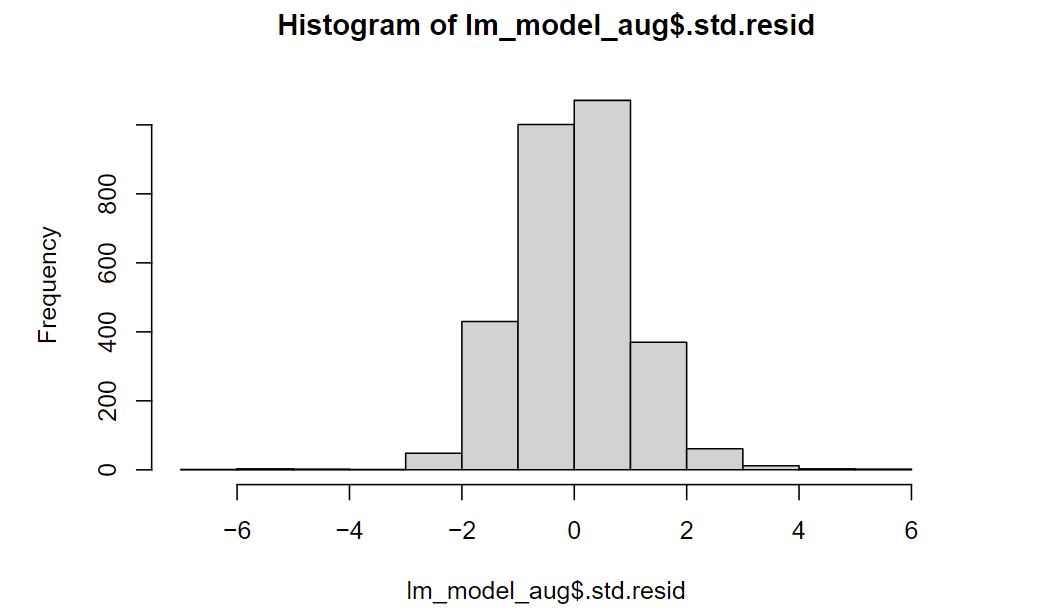
\includegraphics[scale = 0.3]{version2/residual_histo.png} }}%
    \qquad
    \subfloat{{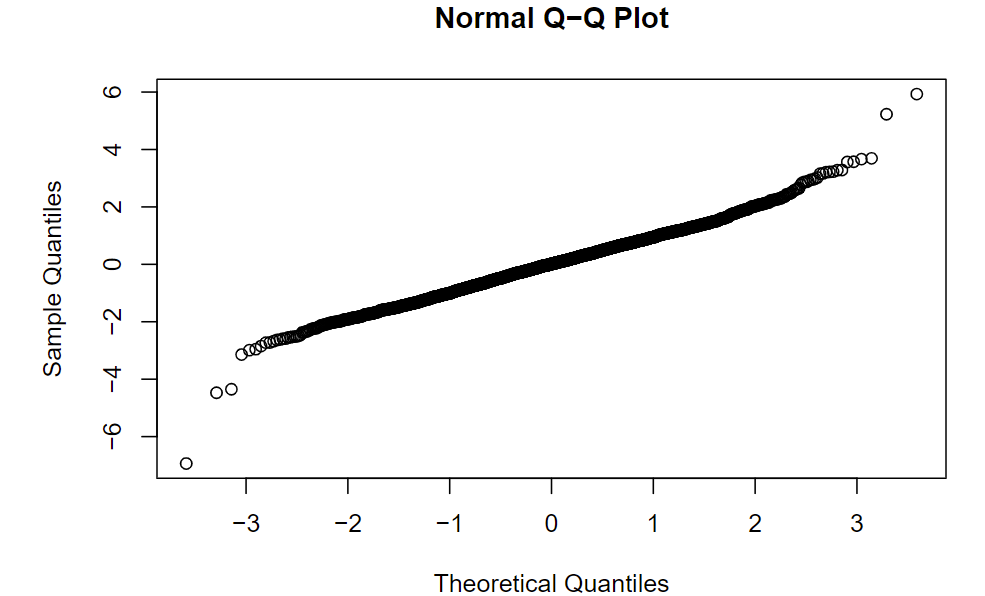
\includegraphics[scale = 0.3]{version2/QQ_plot.png}}}%
    \label{fig:example}%
\end{figure}

We did not conduct a Shapiro-Wilk test, as the test is highly sensitive when we have a large sample size. At large sample sizes, the probability of rejecting the null hypothesis that the residuals are normally distributed becomes extremely large, leading to everything short of perfect normality being rejected by the test. 

Our Breusch-Pagan test for heteroskedascity produced a chi-square statistic that provided strong evidence of heteroskedasticity in our model (BP = 167.5, df = 14). In order to resolve this, we could use White standard errors. Additionally, our Durbin-Watson statistic (1.177) provided strong evidence for autocorrelation. To resolve this, we ran the Cochrane–Orcutt estimation 100 times to purge our standard errors of autocorrelation. Given that we have to fix both problems at the same time though, we opted to use Newey-West standard errors in our model that are robust against both heteroskedascity and autocorrelation. 

Given that our exploratory data analysis (the correlation matrix) provided little evidence of multicollinearity, we were satisfied with concluding that there were no pairwise variables that had concerning levels of multicollinearity. 

Lastly, we attempted to run the Ramsey Reset test again. Our Reset statistic (RESET = 75.65, df1 = 12, df2 = 2972) provided evidence against the logged model, but we were inconclusive on the structure of the correct model. With this, we were left with the following model results.


\begin{table}[!htbp] \centering 
\scriptsize
  \caption{Final Regression Summary} 
  \label{} 
\begin{tabular}{@{\extracolsep{5pt}}lc} 
\\[-1.8ex]\hline 
\hline \\[-1.8ex] 
 & \multicolumn{1}{c}{\textit{Dependent variable:}} \\ 
\cline{2-2} 
\\[-1.8ex] & Coefficients (Robust Standard Errors(HAC SE)) \\ 
\hline \\[-1.8ex] 
 Nominated & 1.556$^{***}$ \\ 
  & (0.283) \\ 
  & \\ 
 log(GrossRevenueTilNom) & 0.088$^{***}$ \\ 
  & (0.011) \\ 
  & \\ 
 CumulativeWeeks & $-$0.054$^{***}$ \\ 
  & (0.003) \\ 
  & \\ 
 WeeklyRank & $-$0.069$^{***}$ \\ 
  & (0.001) \\ 
  & \\ 
 NumTheaters & 0.001$^{***}$ \\ 
  & (0.00001) \\ 
  & \\ 
 Win & $-$0.117$^{***}$ \\ 
  & (0.039) \\ 
  & \\ 
 AAFS & 0.122$^{***}$ \\ 
  & (0.029) \\ 
  & \\ 
 DCR & 0.103$^{***}$ \\ 
  & (0.031) \\ 
  & \\ 
 CMHT & 0.044$^{*}$ \\ 
  & (0.024) \\ 
  & \\ 
 BSHW & $-$0.113$^{***}$ \\ 
  & (0.027) \\ 
  & \\ 
 AMF & 0.096$^{***}$ \\ 
  & (0.034) \\ 
  & \\ 
 log(budget) & $-$0.040$^{***}$ \\ 
  & (0.011) \\ 
  & \\ 
 Nominated:log(GrossRevenueTilNom) & $-$0.112$^{***}$ \\ 
  & (0.016) \\ 
  & \\ 
 Nominated:(CumulativeWeeks) & 0.035$^{***}$ \\ 
  & (0.003) \\ 
  & \\ 
 Constant & 14.652$^{***}$ \\ 
  & (0.201) \\ 
  & \\ 
\hline \\[-1.8ex] 
Observations & 2,999 \\ 
R$^{2}$ & 0.950 \\ 
Adjusted R$^{2}$ & 0.950 \\ 
Residual Std. Error & 0.483 (df = 2984) \\ 
F Statistic & 4,066.637$^{***}$ (df = 14; 2984) \\ 
\hline 
\hline \\[-1.8ex] 
\textit{Note:}  & \multicolumn{1}{r}{$^{*}$p$<$0.1; $^{**}$p$<$0.05; $^{***}$p$<$0.01} \\ 
\end{tabular} 
\end{table} 
\newpage

\section{Empirical Results and Analysis}

Our goal is to estimate the degree to which the explanatory variables discussed in earlier sections are correlated with the weekly box-office revenues in our sample. To do so, we estimate a standard weekly revenue function of the form: 

\begin{align*}
\mathrm{log(WeeklyEarnings)} = \beta_{0}
    &+ \beta_{1}  \mathrm{Nominated} \\
    &+ \beta_{2}  \mathrm{log(GrossRevenueTilNom)} \\
    &+ \beta_{3}  \mathrm{CumulativeWeeks} \\
    &+ \beta_{4}  \mathrm{WeeklyRank} \\
    &+ \beta_{5}  \mathrm{NumTheaters} \\
    &+ \beta_{6}  \mathrm{Win}  \\
    &+ \beta_{7}  \mathrm{AAFS} \\
    &+ \beta_{8}  \mathrm{DCR} \\
    &+ \beta_{9}  \mathrm{CMHT} \\
    &+ \beta_{10}  \mathrm{BSHW} \\
    &+ \beta_{11}  \mathrm{AMF} \\
    &+ \beta_{12}  \mathrm{log(Budget)} \\
    &+ \beta_{13}  \mathrm{Nominated*log(GrossRevenueTilNom)} \\
    &+ \beta_{14}  \mathrm{Nominated*CumulativeWeeks} + \epsilon\\
\end{align*}
\setlength\parindent{0pt}

and the explanatory variables are defined as listed in Table 1. 

\setlength{\parindent}{20pt}

\subsection{Interpretation of Beta Coefficients}

There is little meaning to an intercept coefficient in a case like ours but the best interpretation we can provide is that a movie, in its first week of production, that, by defition, has not been nominated for best picture, has no cumulative gross earnings, has number a cumulative number of weeks of 0, has not been ranked, and is of the W genre, is predicted to earn $e^{14.65}$ or $\$2,303,637.60$ on average.

Based on our model results, holding all else equal, \textit{Nomination} will lead to a predicted increase in the median weekly revenue of a movie by a multiplicative factor of $e^{1.56}$ or $4.759$. Median weekly revenue is predicted to be 4.759 times greater if a movie is nominated for best picture. A nomination also leads to indirect effects via its interaction terms but we could not interpret these concretely as they were dependent on factors that changed week-by-week.

Ceteris paribus, a 10\% increase in \textit{GrossRevenueTilNom} will lead to a predicted increase in the median weekly revenue of a movie by $1.1^{0.088}$ or 0.842\%. Median weekly revenue is predicted to be on average 0.842\% higher if a movie has 10\% greater cumulative gross earnings. A change in \textit{GrossRevenueTilNom} also leads to indirect effects via its interaction term with nominations but we could not interpret these concretely as they were dependent on factors that changed week-by-week.

Ceteris paribus, a 1 week increase in \textit{CumulativeWeeks} will lead to a predicted decrease in the median weekly revenue of a movie by $e^{-0.054}$ or -5.26\%.  Median weekly revenue is predicted to be 5.26\% lower on average if a movie has been out for an additional week. A change in \textit{CumulativeWeeks} also leads to indirect effects via its interaction term with nominations but we could not interpret these concretely as they were dependent on factors that changed week-by-week.

Holding all else equal, a 10\% increase in \textit{budget} will lead to a predicted increase in the median weekly revenue of a movie by $1.1^{-0.04}$ or -0.38\%.  Median weekly revenue is predicted to be on average 0.38\% lower if a movie has a 10\% greater budget.

Holding all else equal, a 1 position increase in \textit{WeeklyRank} will lead to a predicted decrease in the median weekly revenue of a movie by $e^{-0.069}$ or -6.67\%.  Median weekly revenue is predicted to be on average 6.67\% lower if a movie ranking falls by 1 position.

Ceteris paribus, an increase in\textit{NumTheaters} will lead to an increase in the predicted median weekly revenue of a movie by $e^{-0.00067}$ or 0.06\%.  Median weekly revenue is predicted to be on average 0.06\% higher if a movie shows in 1 extra theater.

Holding all else equal, winning best picture is predicted to decrease the median weekly revenue of a movie by $e^{-0.120}$ or -11.31\%. Median weekly revenue is predicted to be on average -11.31\% lower if a movie wins the Oscars. We discuss this result more closely in the next section.

\vspace{\baselineskip} 

For the interpretations of the genres, we will use a Nominated Western movie as the baseline interpretation (for brevity we use the acronyms for our category labels, see section 3.2 for descriptions).

Holding all else equal, a film of the AAFS genre is predicted to increase the median weekly revenue of a movie by $e^{0.12}$ or 12.7\%. Median weekly revenue is predicted to be on average 12.7\% higher if a movie is AAFS as compared to W.

Ceteris paribus, a film of the DCR genre is predicted to increase the median weekly revenue of a movie by $e^{0.10}$ or 10.5\%. Median weekly revenue is predicted to be on average 10.5\% higher if a movie is DCR as compared to W.

Holding all else equal, a film of the CMHT genre is predicted to increase the median weekly revenue of a movie by $e^{0.04}$ or 4.08\%. Median weekly revenue is predicted to be on average 4.08\% higher if a movie is CMHT as compared to W. As this coefficient was statistically insignificant, it had no effect on our model.

Ceteris paribus, a film of the BSHW genre is predicted to decrease the median weekly revenue of a movie by an effect of $e^{-0.11}$ or -10.41\%. Median weekly revenue is predicted to be on average 10.41\% lower if a movie is BSHW as compared to W.

Ceteris paribus, a film of the AMF genre is predicted to increase the median weekly revenue of a movie by $e^{0.09}$ or 9.42\%. Median weekly revenue is predicted to be on average 9.42\% higher if a movie is AMF as compared to W.


\subsection{Analysis}

Our results indicate that best picture Oscar \textit{nominations} have a positive effect on weekly revenues, but a winning has a negative. While this may seem odd at first sight, the negative value for a win makes sense considering our model specification. A key feature of our model is that are dealing with \textit{weekly} revenues, and we take into consideration the \textit{time} a movie has been screening in theaters. A possible explanation for why a Oscar win is negatively correlated to weekly revenues may be attributed to the fact that nominated films are in theaters for some time before the Oscars announcement. Nominated films have already built up a certain economic traction; if a movie has already earned substantial revenues before winning the Best Picture Award, there is less room to grow. We can reasonably infer that the nomination gives weekly earnings a slight ``boost" with consumers who did not watch the movie prior to nominations. By the time Oscar wins are announced, many people will have seen the movie already. Because movies are experience goods, it is unlikely that even the most ardent fans will watch the same movie in theaters multiple times. As a result, weekly weekly revenues dwindle afterwards. Thus, demand for a film falls by the time the Oscar awards winner for best picture is announced. This is one possible explanation for a negative coefficient on \emph{Winning}.

A surprising result was a negative correlation for budget. We believe that the negative correlation between budget and earnings can attributed to a form of omitted variable bias. Due to a lack of access to the appropriate data we were unable to split up total movie budget into its components: advertising, costs of actors, etc.. We believe each of these have dramatically different effects on earnings.

As for genres, the effects seem in-line with our expectations that biographic movies and the-like tend to under-perform in the box-office due to their limited appeal to a wider audience.

We additionally found it interesting that the estimated coefficient for nomination was positive but the estimated coefficient for the interaction between nomination and log(GrossRevenueTilNom) was negative. In particular, we propose that the nomination's effect on a movie is affected by its total earnings so far, with higher total earnings leading to smaller (and in this case negative) gains to the movie's weekly revenue. This makes sense, given that most popular movies that get nominated already have been viewed by most people, and thus do not get any boost from the nomination or win.


\subsection{Further Limitations}

The Ramsey Reset Test provides clear evidence that our model has room for improvement. With stronger economic training and theory as well as further statistical tools we could begin to create a model which had a structure that better fits the data: our Reset test suggested that our logged linear model does not do that. However, we don't know what model would be a better alternative. 

Further, we were working with time-series data but did not have the ability to use time series models, which limited the set of tools for model building to multi-variable regression analysis. For further study, we could use a LSTM model that could better work with time-series data. 


Our dataset also includes notable outliers such as \textit{Avatar}. For such blockbuster films, it is difficult to say whether awards influence success, or whether the Academy goes with the flow. \textit{Avatar}, for example, made 140 million USD in the first week alone. Due to complications in defining an exact threshold for excluding movies, however, we did not remove these observations — which may have skewed our results towards higher earnings. 






\section{Conclusion}
We conclude that an Oscar Best Picture win is a combination of its nomination, win, and the interaction between its nomination and total earnings till that date. We posit that as the nomination already provides a significant boost in weekly revenue, a win will not bring any additional boosts and that it is entirely possible that the model only captures the effects of the downtrend post-win. Our final thoughts on what a Best Picture Oscar win is worth would be an estimated 4.22 times increase in weekly revenues multiplied by the interaction between nominations and cumulative weeks and nominations and the log of cumulative gross revenue.

Although our measure of a movie’s ‘success’ is weekly box office revenues, it is also important to acknowledge that the Academy does not blindly endorse the masses, given the Academy’s own proclamation that “excellence in filmmaking is the only factor" in casting votes. The votes are cast by, namely, members of the Academy who comprise of “gifted and skilled artists and craftsmen in the motion picture world” -- 8,100 members as of 2019). The panel of judges are chosen on an invite-only basis; the exact criterion is not known to the public. As such, commercial success and Oscar wins may only be associated to the extent that these supposed experts and moviegoers share the same taste. 

For extensions to this analysis, we note that the movie industry has undergone structural changes during the time frame 2000-2019 for which we collected our data. With the rise of Netflix and other streaming services, box office numbers measuring ticket sales are incomplete and don't show the full picture for the demand of a movie. Nowadays, consumers can enjoy a newly released movie in the comfort of their homes. For a more comprehensive analysis in future studies, we could look at user data from streaming services. 

Another topic of future investigation would be to explore the factors that affect Oscar nominations and wins, that is, treating them as endogenous rather than exogenous variables . This could allow to identify the extent to which a certain variables, like genre, could improve the odds of winning an Oscar. 


\newpage
\section*{References}
\leftskip 0.3in
\parindent -0.3in

\noindent 
 
 Bristor, J. (1990), "Enhanced Explanation of Word of Mouth Communications: The Power of Relationships," in Research in Consumer Behavior, E.C. Hirschman, ed. Greenwich, CT: JAI Press, 51-8

Deuchert,, E., Adjmah, K., & Pauly, F. (2005). For Oscar Glory or Oscar Money? Journal of Cultural Economics, 29(3), 159–176. http://www.jstor.org/stable/41810887 

Elberse, A. (2007). The Power of Stars: Do Star Actors Drive the Success of Movies? Journal of Marketing, 71(4), 102–120. http://www.jstor.org/stable/30164000 

Einav, L. (2007). Seasonality in the U.S. Motion Picture Industry. The RAND Journal of Economics, 38(1), 127–145. http://www.jstor.org/stable/25046296 
 
Ginsburgh, V. (2003). Awards, Success and Aesthetic Quality in the Arts. The Journal of Economic Perspectives, 17(2), 99–111. http://www.jstor.org/stable/3216859 

Harrison-Walker, L. Jean (2001), "The Measurement of Word-of- Mouth Communication and an Investigation of Service Quality and Customer Commitment as Potential Antecedents," Journal of Services Marketing. 

Levy E. (2001) Oscar Fever: The History and Politics of the Academy Awards (The Continuum International Publishing Group, New York). 

Liu, Yong (2006), "Word of Mouth for Movies: Its Dynamics and Impact on Box Office Revenue," Journal of Marketing, 70 (July), 74-89

Liu, A., Liu, Y., & Mazumdar, T. (2014). Star power in the eye of the beholder: A study of the influence of stars in the movie industry. Marketing Letters, 25(4), 385–396. http://www.jstor.org/stable/24571121

Moon, S., Bergey, P. K., & Iacobucci, D. (2010). Dynamic Effects among Movie Ratings, Movie Revenues, and Viewer Satisfaction. Journal of Marketing, 74(1), 108–121. http://www.jstor.org/stable/20619083 

Pennington, J. W. (2007). The history of sex in American film. Westport: Praeger.


Redondo, I., and Morris B. Holbrook. “Modeling the Appeal of Movie Features to Demographic Segments of Theatrical Demand.” Journal of Cultural Economics 34, no. 4 (2010): 299–315. http://www.jstor.org/stable/41811062.
 
Sawhney, M. S., & Eliashberg, J. (1996). A Parsimonious Model for Forecasting Gross Box-Office Revenues of Motion Pictures. Marketing Science, 15(2), 113–131.\\ http://www.jstor.org/stable/184189




\end{document}
